\documentclass[12pt,a4paper]{article}

\setlength{\textwidth}{165mm}
\setlength{\textheight}{240mm}
\setlength{\parindent}{0mm} % S{\aa} meget rykkes ind efter afsnit
\setlength{\parskip}{\parsep}
\setlength{\headheight}{0mm}
\setlength{\headsep}{0mm}
\setlength{\hoffset}{-2.5mm}
\setlength{\voffset}{0mm}
\setlength{\footskip}{15mm}
\setlength{\oddsidemargin}{0mm}
\setlength{\topmargin}{0mm}
\setlength{\evensidemargin}{0mm}
\usepackage{multicol}
\usepackage{blindtext}
\usepackage[all]{xy}
\usepackage{graphicx}    % For grafik (billederfiler)
\usepackage[T1]{fontenc} % For at blande \textsc{} med \textbf{}
\usepackage[utf8]{inputenc}
\usepackage{amsfonts,amsmath,amssymb}
\usepackage{eucal}
\usepackage{enumerate}  
\usepackage{hyperref}
\usepackage{url}
\usepackage{mathptmx}
\usepackage{multirow}
\usepackage[dvipsnames,usenames]{color}
\usepackage{tabularx,colortbl,xcolor}
\usepackage{listings}
\usepackage{color}
\usepackage{amsmath}
\usepackage{xcolor}

\definecolor{KU-red}{RGB}{144,26,30} 
\definecolor{dkgreen}{rgb}{0,0.6,0}
\definecolor{gray}{rgb}{0.5,0.5,0.5}
\definecolor{mauve}{rgb}{0.58,0,0.82}

\lstset{frame=tb,
  language=Java,
  aboveskip=3mm,
  belowskip=3mm,
  showstringspaces=false,
  columns=flexible,
  basicstyle={\small\ttfamily},
  numbers=none,
  numberstyle=\tiny\color{gray},
  keywordstyle=\color{blue},
  commentstyle=\color{dkgreen},
  stringstyle=\color{mauve},
  breaklines=true,
  breakatwhitespace=true,
  tabsize=3}

\DeclareSymbolFont{usualmathcal}{OMS}{cmsy}{m}{n}
\DeclareSymbolFontAlphabet{\mathcal}{usualmathcal}
\DeclareSymbolFont{letters}{OML}{txmi}{m}{it}

\DeclareMathSymbol{\alpha}{\mathord}{letters}{"0B}
\DeclareMathSymbol{\beta}{\mathord}{letters}{"0C}
\DeclareMathSymbol{\gamma}{\mathord}{letters}{"0D}
\DeclareMathSymbol{\delta}{\mathord}{letters}{"0E}
\DeclareMathSymbol{\epsilon}{\mathord}{letters}{"0F}
\DeclareMathSymbol{\zeta}{\mathord}{letters}{"10}
\DeclareMathSymbol{\eta}{\mathord}{letters}{"11}
\DeclareMathSymbol{\theta}{\mathord}{letters}{"12}
\DeclareMathSymbol{\iota}{\mathord}{letters}{"13}
\DeclareMathSymbol{\kappa}{\mathord}{letters}{"14}
\DeclareMathSymbol{\lambda}{\mathord}{letters}{"15}
\DeclareMathSymbol{\mu}{\mathord}{letters}{"16}
\DeclareMathSymbol{\nu}{\mathord}{letters}{"17}
\DeclareMathSymbol{\xi}{\mathord}{letters}{"18}
\DeclareMathSymbol{\pi}{\mathord}{letters}{"19}
\DeclareMathSymbol{\rho}{\mathord}{letters}{"1A}
\DeclareMathSymbol{\sigma}{\mathord}{letters}{"1B}
\DeclareMathSymbol{\tau}{\mathord}{letters}{"1C}
\DeclareMathSymbol{\upsilon}{\mathord}{letters}{"1D}
\DeclareMathSymbol{\phi}{\mathord}{letters}{"1E}
\DeclareMathSymbol{\chi}{\mathord}{letters}{"1F}
\DeclareMathSymbol{\psi}{\mathord}{letters}{"20}
\DeclareMathSymbol{\omega}{\mathord}{letters}{"21}
\DeclareMathSymbol{\varepsilon}{\mathord}{letters}{"22}
\DeclareMathSymbol{\vartheta}{\mathord}{letters}{"23}
\DeclareMathSymbol{\varpi}{\mathord}{letters}{"24}
\DeclareMathSymbol{\varrho}{\mathord}{letters}{"25}
\DeclareMathSymbol{\varsigma}{\mathord}{letters}{"26}
\DeclareMathSymbol{\varphi}{\mathord}{letters}{"27}
\DeclareMathSymbol{\Gamma}{\mathord}{letters}{"00}
\DeclareMathSymbol{\Delta}{\mathord}{letters}{"01}
\DeclareMathSymbol{\Theta}{\mathord}{letters}{"02}
\DeclareMathSymbol{\Lambda}{\mathord}{letters}{"03}
\DeclareMathSymbol{\Xi}{\mathord}{letters}{"04}
\DeclareMathSymbol{\Pi}{\mathord}{letters}{"05}
\DeclareMathSymbol{\Sigma}{\mathord}{letters}{"06}
\DeclareMathSymbol{\Upsilon}{\mathord}{letters}{"07}
\DeclareMathSymbol{\Phi}{\mathord}{letters}{"08}
\DeclareMathSymbol{\Psi}{\mathord}{letters}{"09}
\DeclareMathSymbol{\Omega}{\mathord}{letters}{"0A}
\DeclareMathSymbol{\upGamma}{\mathalpha}{operators}{"00}
\DeclareMathSymbol{\upDelta}{\mathalpha}{operators}{"01}
\DeclareMathSymbol{\upTheta}{\mathalpha}{operators}{"02}
\DeclareMathSymbol{\upLambda}{\mathalpha}{operators}{"03}
\DeclareMathSymbol{\upXi}{\mathalpha}{operators}{"04}
\DeclareMathSymbol{\upPi}{\mathalpha}{operators}{"05}
\DeclareMathSymbol{\upSigma}{\mathalpha}{operators}{"06}
\DeclareMathSymbol{\upUpsilon}{\mathalpha}{operators}{"07}
\DeclareMathSymbol{\upPhi}{\mathalpha}{operators}{"08}
\DeclareMathSymbol{\upPsi}{\mathalpha}{operators}{"09}
\DeclareMathSymbol{\upOmega}{\mathalpha}{operators}{"0A}

\newcommand{\hhemail}[1]{\textsf{#1}}
\newcommand{\hhurl}[1]{{\color{blue}\url{#1}}}

\begin{document}
	
	\begin{minipage}[b]{1.0\linewidth} 
				
\includegraphics[height=50mm]{KULogo.pdf}
		
		\vspace*{-16ex}
		\vspace {35ex}
		\begin{center}
			{\huge \bf Project: Beetle} \vspace*{4ex} \\
			{\large 13. maj 2015}\\
			\vspace*{2ex}
			qzj710 - 121095 - Enes Golic \\
			rpc308 - 070493 - Yunus Emre Okutan \\
			cbh239 - 250594 - Casper Lützhøft Christensen \\
			mhb558 - 250795 - Tor-Salve Dalsgaard\\
			\vspace*{1ex}
			Instructor - Kasper Passov
			
		\end{center}
	\end{minipage}
	
\newpage
\tableofcontents

\newpage
\section{Introduction}
\subsection{Abstract}
Our project is a search-engine attached to a database containing insects as entries, and is to be provided to our client the University of Hamburg (from here on abbreviated ”UH”).
German law dictates that a university must make all research conducted publicly available to anyone seeking the knowledge – it is in this context our project has been requested.
Through research UH's entomology department has established a catalogue of information on different specimen of insect, including their names, species, subspecies, genus and pictures of its anatomy and location.
We will be using this information as attributes in our database, which will feature the specimen of insect as the entry.
The search-engine we create will then allow a visitor to input a search-term, which will be tried against any of the attributes in the database and return all entries with an attribute matching.
In addition, the project will feature an advanced search-engine, which will allow a visitor to input search-terms to be matched against specific attributes, rather than against every attribute.
Furthermore, UH must be able to update the database themselves, we will therefore provide an administrator control panel – protected by a login system - where entries can be added and deleted.
Because some of the specimen of insects recorded in the database are potentially threatened by extinction, UH has also requested entries can be made not publicly available.
We will therefore create a function to hide specific entries from ordinary visitors, but allow the administrator to create temporary users that can view it.
The project will be created using PHP, Javascript and MySQL, and will feature the search-engine, the advanced search-engine, the temporary user copies of the 2 former mentioned as well as an administrator control panel.
\newpage

\section{FACTOR}
\subsection{Functionality}
Allow visitors to use the 2 search-functions, basic and advanced, to search through a database
of insect-entries with data collected by the University of Hamburg. 
Allow the administrator with login-credentials to remove or add new entries to the database.
Allow the adminstrator to create temporary users for aspiring scientists or enthusiasts, so that they can view entries that cannot be publicly available (because they might be facing extinction).
Allow temporary users to use a log into the website and view every insect in the database. 
\subsection{Application-domain}
The product is to be available to everybody seeking to use it in the pursuit of knowledge – this means students, researchers, professors and anonymous visitors alike.
Only the administrator however will be able to make changes to the database, and only users who are given login credentials will be able to view an insect's location.
\subsection{Conditions}
This product is being developed as part of the course PKSU at the University of Copenhagen. It is therefore by us completely voluntarily developed and no gain on our side apart from experience is being received. 
The product must be freely available, on the University of Hamburg's website, to anyone who wishes access to the information stored within. The product is not to be used to generate any profit whatsoever, its only purpose is the distribution of knowledge.
\subsection{Technology}
The product is developed through the server-side language PHP, client-side language Javascript and the database-management-language MySQL. As such, nothing but a computer and an internet-connection has been required in order to develop it.
Due to this, the product can run in any browser and on any application (computer/phone) with an internet connection.
\subsection{Objects}
The product consists of a webpage containing the search-engine. From the standard search-engine you can either, as an anonymous viewer, enter the advanced search-engine or, as an employee, login to the editting interface using provided login credentials.
\subsection{Responsibility}
The responsibility of the product is, through a search-engine, to ensure free and public access to research conducted by the University of Hamburg. 
\newpage
\section{Program Specifications}
\subsection{Functional and Non-Functional Requirements}

If we refer to the abstract outlining the program's specifications, we get a general feel of the architecture of the software and how it is going to work. Drawing on those points we can, for the sake of overview, specify functional and non-functional requirements for the program.\\

{\bf Functional Requirements}
\begin{itemize}
	\item The product must offer a search-option that returns any and every entry that contains an attribute that matches the search input.
	\item The product must offer a search-option that allows matching of specific search-inputs to specific attributes and return any and every entry that matches the terms in their specific attributes.
	\item The database must allow the creation of new entries, editing of existing entries and deletion of existing entries.
	\item The database must be unable to be edited by anyone save the authorised employees.
	\item A fitting message must be displayed if no matching entries are found.
	\item The database must allow the creation of new entries and deletion of existing entries.
	\item The database must only be editable by the administrator of the site.
	\item The administrator must be able to create temporary users that can view entries that are not otherwise displayed due to being threatened.\\
\end{itemize}
{\bf Non-Functional Requirements}
\begin{itemize}
	\item The search-engine must be developed in PHP so it can run on their website in any browser with no additional requirements.
	\item The method of editing the database must be simple enough for people without pre-existing IT skills to use it.
	\item The product in its finished state must look nice and fit with the colour-scheme already present on the University of Hamburg's website.
\end{itemize}
\newpage
\subsection{Use Case Model}
\vskip\medskipamount % or other desired dimension
\leaders\vrule width \textwidth\vskip0.4pt % or other desired thickness
\vskip\medskipamount % ditto
\nointerlineskip
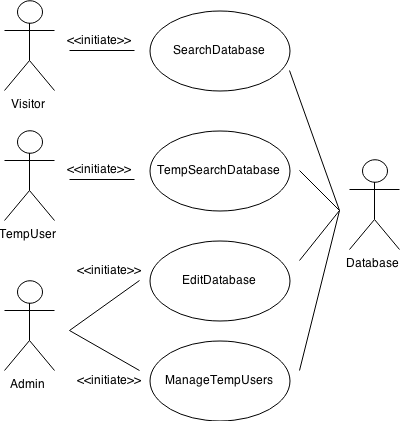
\includegraphics[height=120mm]{UseCase.png}

{\bf SearchDatabase}\\ 
Visitors can use the search-engine by inputting the term(s) they wish to try against the database and the matching results displayed.
Searching the database requires no logging in.\\
{\bf TempSearchDatabase}\\
Temporary users can use the search-engine that will also display the location of the entry. They are required to login to access this functionality.\\
{\bf EditDatabase}\\
An administrator can edit the database by adding or removing entries from it, as long as he is logged into the control panel.\\
{\bf ManageTempUsers}\\
An administrator can also create logins for temporary users, so that they can view information that is not supposed to be publicly available.\\
He can also delete these logins when deemed appropriate.\\
\vskip\medskipamount % or other desired dimension
\leaders\vrule width \textwidth\vskip0.4pt % or other desired thickness
\vskip\medskipamount % ditto
\nointerlineskip
The figure above is a use-case model, depicting the possibilities and permissions of the various different users the site can encounter.\\
For instance any visitor will be able to use the frontpage search-engine.
If granted a login by the administrator, you can log in as a temporary user and use a search-engine that will also display the location.\\
The administrator can edit the database and also manages the temporary users.
\newpage

\subsection{Specific Use Cases}

With the use case model created, we have an overview of the functional architecture of the website. With that in mind, we can explore some of the specific cases a bit further:\\

$\begin{array}{ll}
\hline
\text{Use Case Name}	& \text{SearchDatabase}\\
\hline
\text{Participating
	actors}	& \text{Initiated by Visitor}\\
\hline
\text{Flow of events}	& \text{1. A visitor enters the website.}\\
& \text{2. The visitors enters the search-term into the search-field and presses send.} \\
& \text{3. The matching results are displayed.}\\
\hline
\text{Entry condition}	& \text{None}\\
\hline
\text{Exit conditions}	& \bullet \text{Anonymous exits the site.}\\
& \bullet \text{Anonymous submits a new search term.}\\
\hline
\end{array}$
\\

The above use case is the ordinary search of the database. It showcases in detail the specifics of the use case by displaying who initiates it, who, if any, it communicates with, the flow of the case itself as well as any conditions necessary.
We will now also inspect 2 other use cases:\\

$\begin{array}{ll}
\hline
\text{Use Case Name}	& \text{ManageTempUsers}\\
\hline
\text{Participating
	actors}	& \text{Initiated by Administrator}\\
& \text{Communicates with Database}\\
& \text{Communicates with TempUser}\\
\hline
\text{Flow of events}	& \text{1. The Administrator enters the website.}\\
& \text{2. The Administrator logs into the control-panel using his login credentials.} \\
& \text{3. The Administrator creates or removes a temporary user.}\\
\hline
\text{Entry condition}	& \text{Must have Administrator credentials.}\\
\hline
\text{Exit conditions}	& \bullet \text{Administrator exits the site.}\\
& \bullet \text{Administrator logs out of control-panel.}\\
\hline
\end{array}$\\
\\
This is the case of the Administrator either creating or deleting a temporary user. This is, of course, only available to the administrator with credentials.\\

$\begin{array}{ll}
\hline
\text{Use Case Name}	& \text{EditDatabase}\\
\hline
\text{Participating
	actors}	& \text{Initiated by Administrator}\\
& \text{Communicates with Visitor}\\
& \text{Communicates with Database}\\
& \text{Communicates with TempUser}\\
\hline
\text{Flow of events}	& \text{1. The Administrator enters the website.}\\
& \text{2. The Administrator logs into the control-panel using his login credentials.} \\
& \text{3. The Administrator makes the desired changes to the database}\\
\hline
\text{Entry condition}	& \bullet \text{Must have Administrator credentials.}\\
\hline
\text{Exit conditions}	& \bullet \text{Administrator exits the site.}\\
& \bullet \text{Administrator logs out of control-panel.}\\
\hline
\end{array}$
\\

As with the case preceeding it, administrator credentials are also necessary to edit the database.
\newpage

\subsection{Class-diagram}

In order to grant an overview of the software-architecture, a class-diagram has been created:

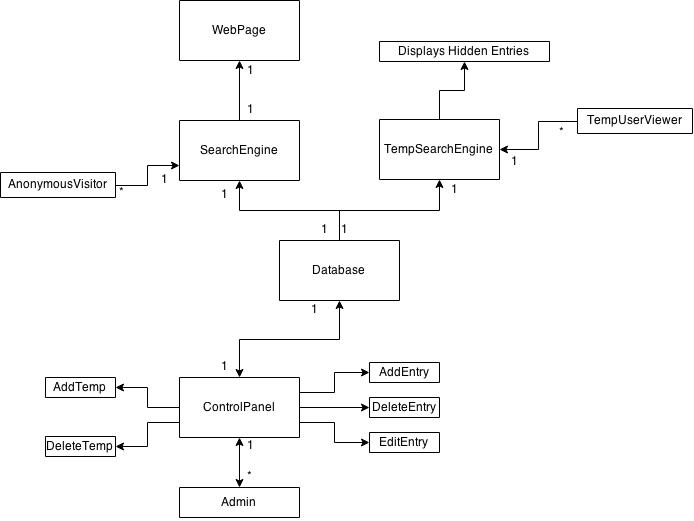
\includegraphics[height=110mm]{ClassDiagram.png}

The class diagram shows the elements of our website and how they are connected. Our Webpage has two search engines, one for simple search statements, and for a more advanced approach an advanced search. These two can be used by an anonymous visitor, but in addition the admin is using the same search engine in his control panel. The search engines are connected to a database which holds all the entities, can create, edit or remove entries in the database, hence the pictures that pop up when searched for. The database can't do these things by itself, that is why we have made a control panel in which the admin can change the entries, but the admin can also add guest users to the system. Since our project revolves around special butterflies and insects, our goal is to preserve the nature by not giving out details to anyone. Some of the insects are endangered, meaning that the university now have the opportunity to permit certain users access, by creating a temporary user for them in the control panel. These users can only be added or deleted. The admin is connected to all of this, and as we stated earlier the admin takes use of the search engine to make it easier for himself to check for a specific species, subspecies or genus. Instead of looking through of a list a maybe 100 entries, he can search for the specific genus he wishes to look for. In order to make as many entries available for the public, we have added a box which the owners can tick, and telling the database that it can only be accessed by a temporary user created in the system. In our class diagram we have stated this special incident as being a parametre for the temporary users: "Display Hidden Entries".
\newpage
\subsection{BCE}

To provide an easy reference-point for the different objects in our product and their respective responsibilities, a BCE has been created to effectively sort those objects into their representative categories.

\begin{gather*}
\begin{bmatrix}
\textbf{B}&\textbf{C}&\textbf{E}\\
Buttons&Search&Entries\\
Textfields&Advanced Search&Images\\
Headline&TempUserSearch\\
Background&TempUserAdvSearch\\
 &ImageClick\\
 &Edit\\
\end{bmatrix}
\end{gather*}\\
\textbf{Boundary:}\\

Everything a user can see is a boundary object. In our case the buttons, also the text fields, the headline and the grey background.\\


\textbf{Entity:}\\

The entities here are all the information from the database, as well as the images that represent a specific set of information (an entry).\\

\textbf{Control:}\\

The search-button grabs the text input into the search-field and matches the term against the database.
The advanced search-button is similar except that it has 4 fields in which a user can match a term against specific attributes. \\
Clicking on an image will take the user to a full-scale version of the image clicked.\\
Finally we have the edit button that allows an employee to change the entries in the database, or add/remove entries.
These are all control objects as they control one or more parts of the website's functionality.\\
In some cases when the user is allowed additional access through having a username and password, the user can then view the TempUserSearch and TempUserAdvSearch, which allow them to see the endangered objects.

\newpage
\subsection{Sequence-diagram}
We've already previously established different use cases relating to the project. Through these we can create sequence-diagrams illustrating them:
\\

{\bf Use Case: SearchDatabase}\\

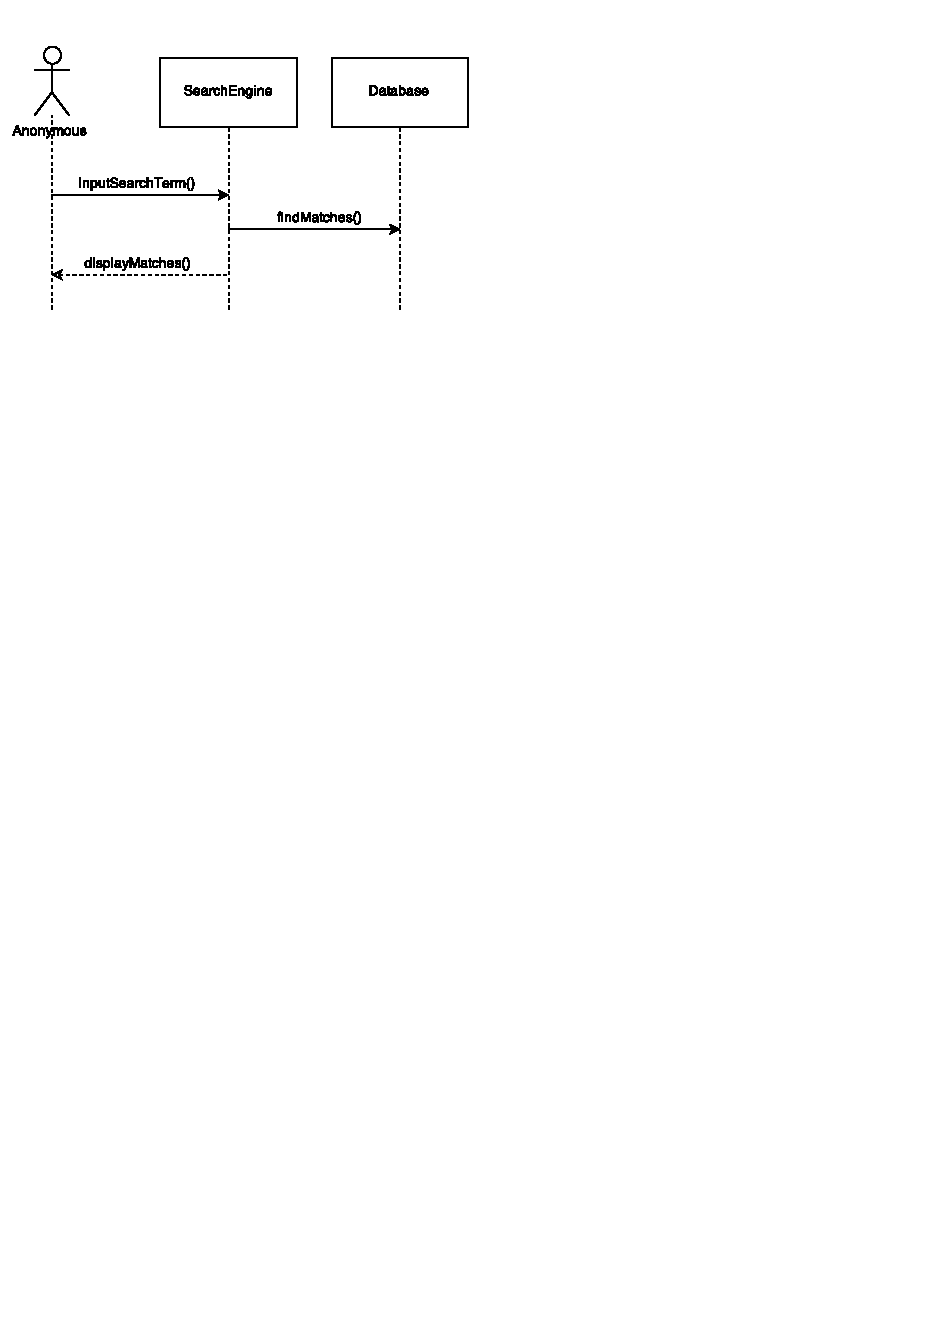
\includegraphics[height=92mm]{Sequence1.pdf}

{\bf Use Case: ManageTempUsers}\\

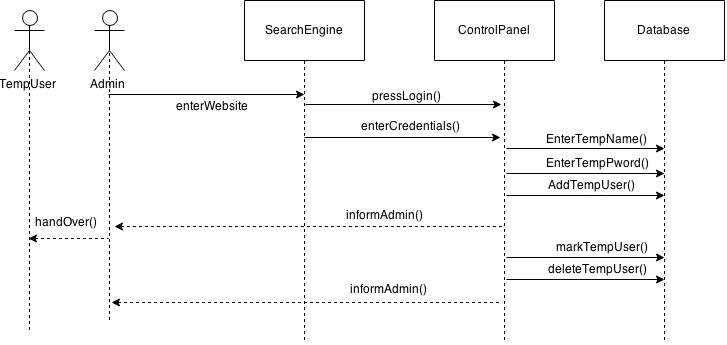
\includegraphics[height=86mm]{Sequence2.jpg}
The idea is that this sequence diagram works with the recently added tempuser. The admin enters the searchengine, where he enters the controlPanel. He can add the name, password and in the end the temporary user to the database. The admin is then informed of the newly added user, which he then can handover to the temporary user.\\
The admin can then later mark the created temporary user, and delete it. 
\\

{\bf Use Case: EditDatabase}\\

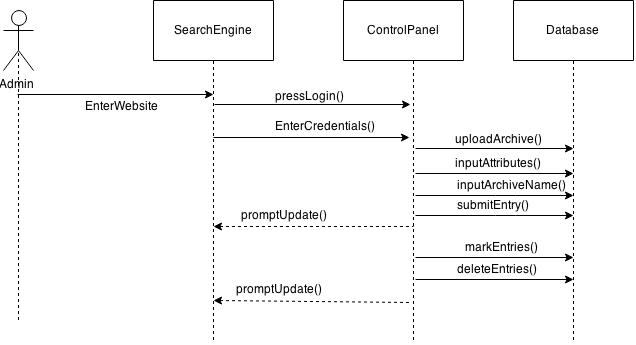
\includegraphics[height=92mm]{Sequence3.jpg}

\newpage

\section{System Design}
\subsection{Current Progress}

The Prototype of our product can be found and accessed at: \url{http://echiever.de/ProjectBeetle/Prototype3/prototype3.php}
\subsection{Summary}

At the current-stage of our product everything is fully functional.\\
The database consists of insect-entries, with order, family, genus, species, subspecies, description and the name of the .zip archive containing the high-resolution zoomify image of the insect as attributes.
Both the search-function and the advanced search-function are fully functional, and a method of displaying all existing entries in the database has been added (by simply searching for no term).
The database is now editable by either adding or deleting entries.\\
To add an entry you must now first upload an archive containing the zoomify image of an insect, and thereafter enter the appropriate information into its respective attributes, as well as enter the name of the archive which you uploaded.
Deleting an entry is done simply by marking a checkbox and clicking a delete-button.
At this point, all functional requirements have been fulfilled, and our work going forward is:
\begin{itemize}
\item Improve the design to better match that of the University of Hamburg's existing website
\item Implement any further wises the client may have
\end{itemize}
\newpage
\section{Testing}
\subsection{Search-engine test}

Testing the current edition of the product has gone to show that every of our newly implemented changes work as intended. We did however locate one problem, which is that logging out currently does appropriately delete the cookie responsible for checking whether you're logged in or not, and simply pressing 'return' after having logged out, will not re-prompt you for your credentials.

As for the current search, it now works with our updated database that includes the zoomify images.\\
The current search-able words in the normal search-engine are:

\begin{itemize}
	\item testFamily
	\item Sterrha
	\item Eilicrinia
\end{itemize}

As for testing the advanced search-engine, the following combination of terms and letters allow for full showing of its functionality.
\\\\
$
\begin{array}{c|c|c}
Order & Contains & stOr \\ 
Family & Starts with & test \\ 
Genus & Ends with & rha \\ 
Species & Contains & cord
\end{array}
$
\\

More in-depth descriptions of the various conducted tests are available as annexes at the end of the report.

\newpage
\section{Interaction and Design}
\subsection{Design}

In order to showcase the unit-interface of the product, a series of screenshots have been provided.

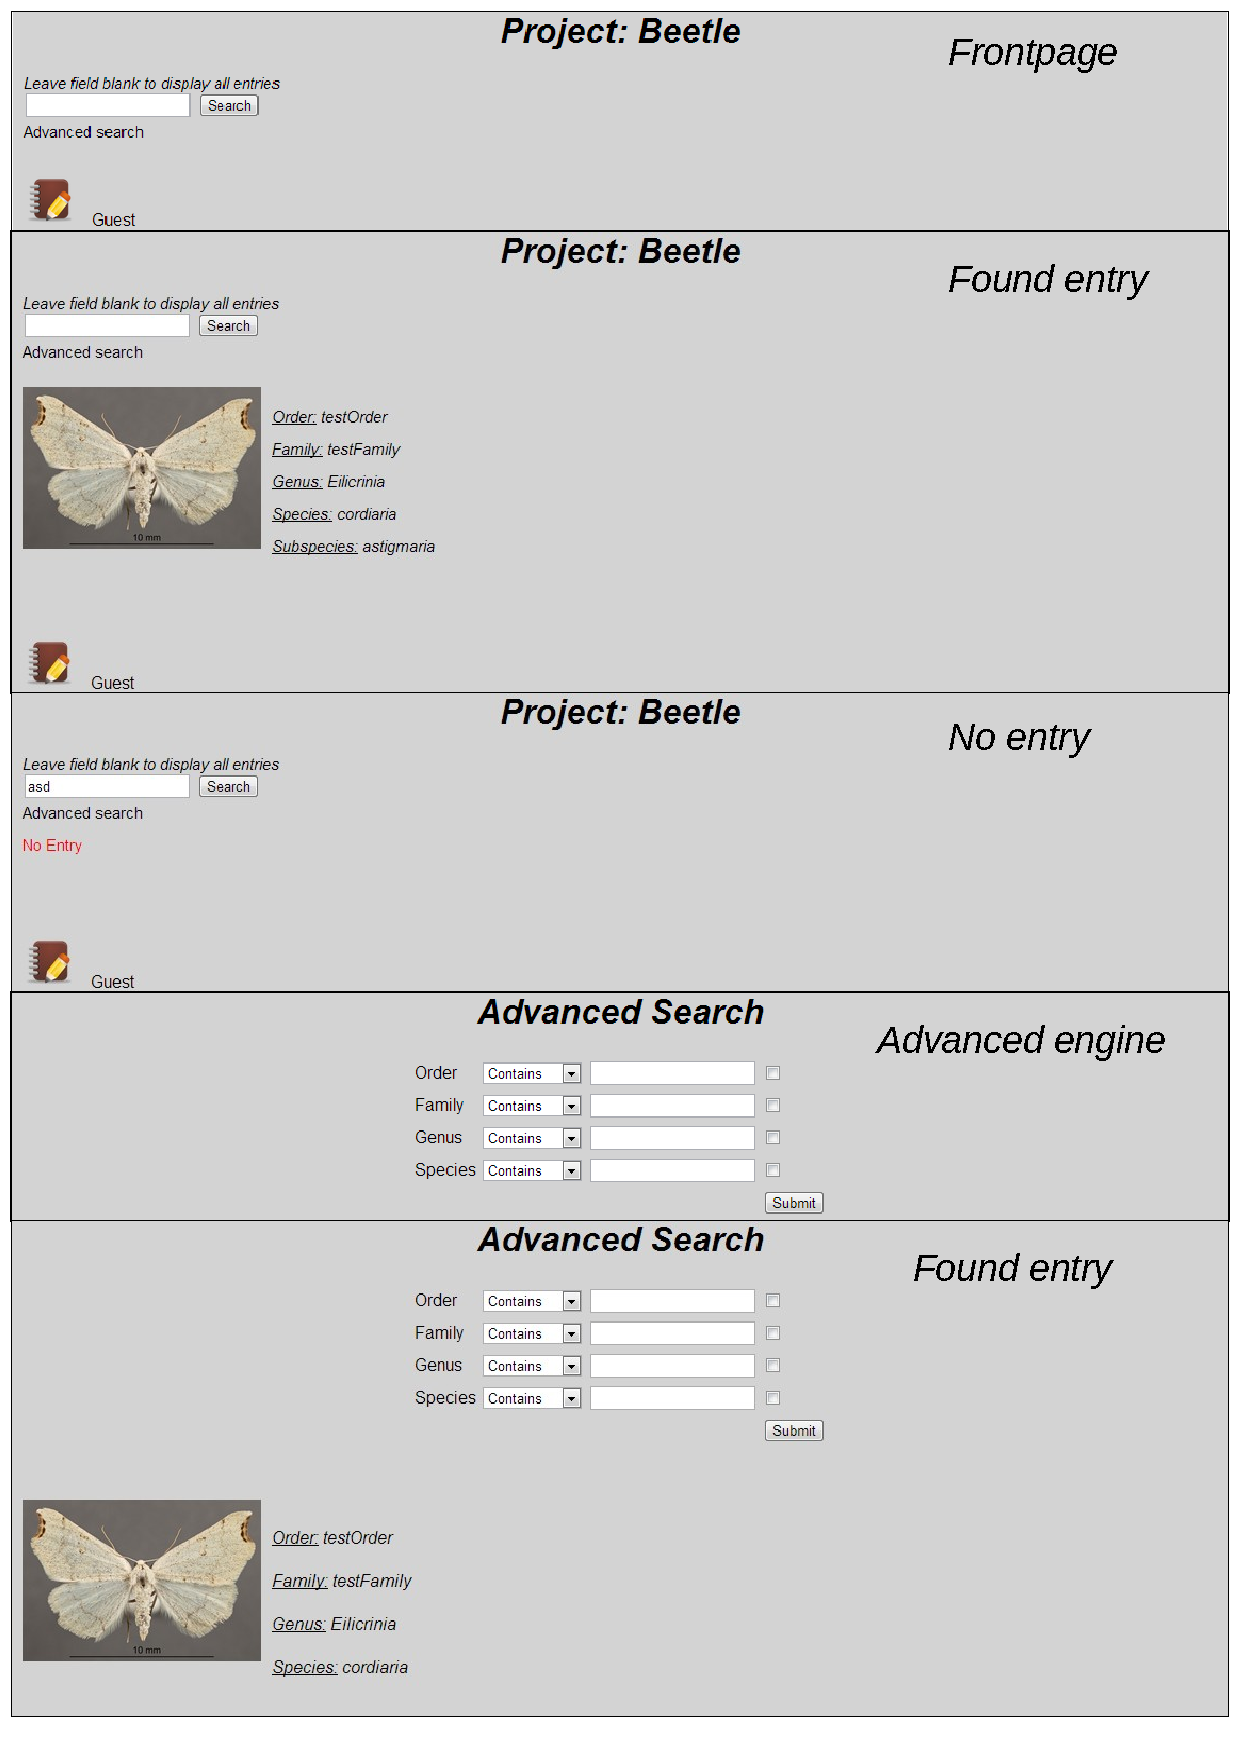
\includegraphics[height=205mm]{UI1.pdf}
\newpage
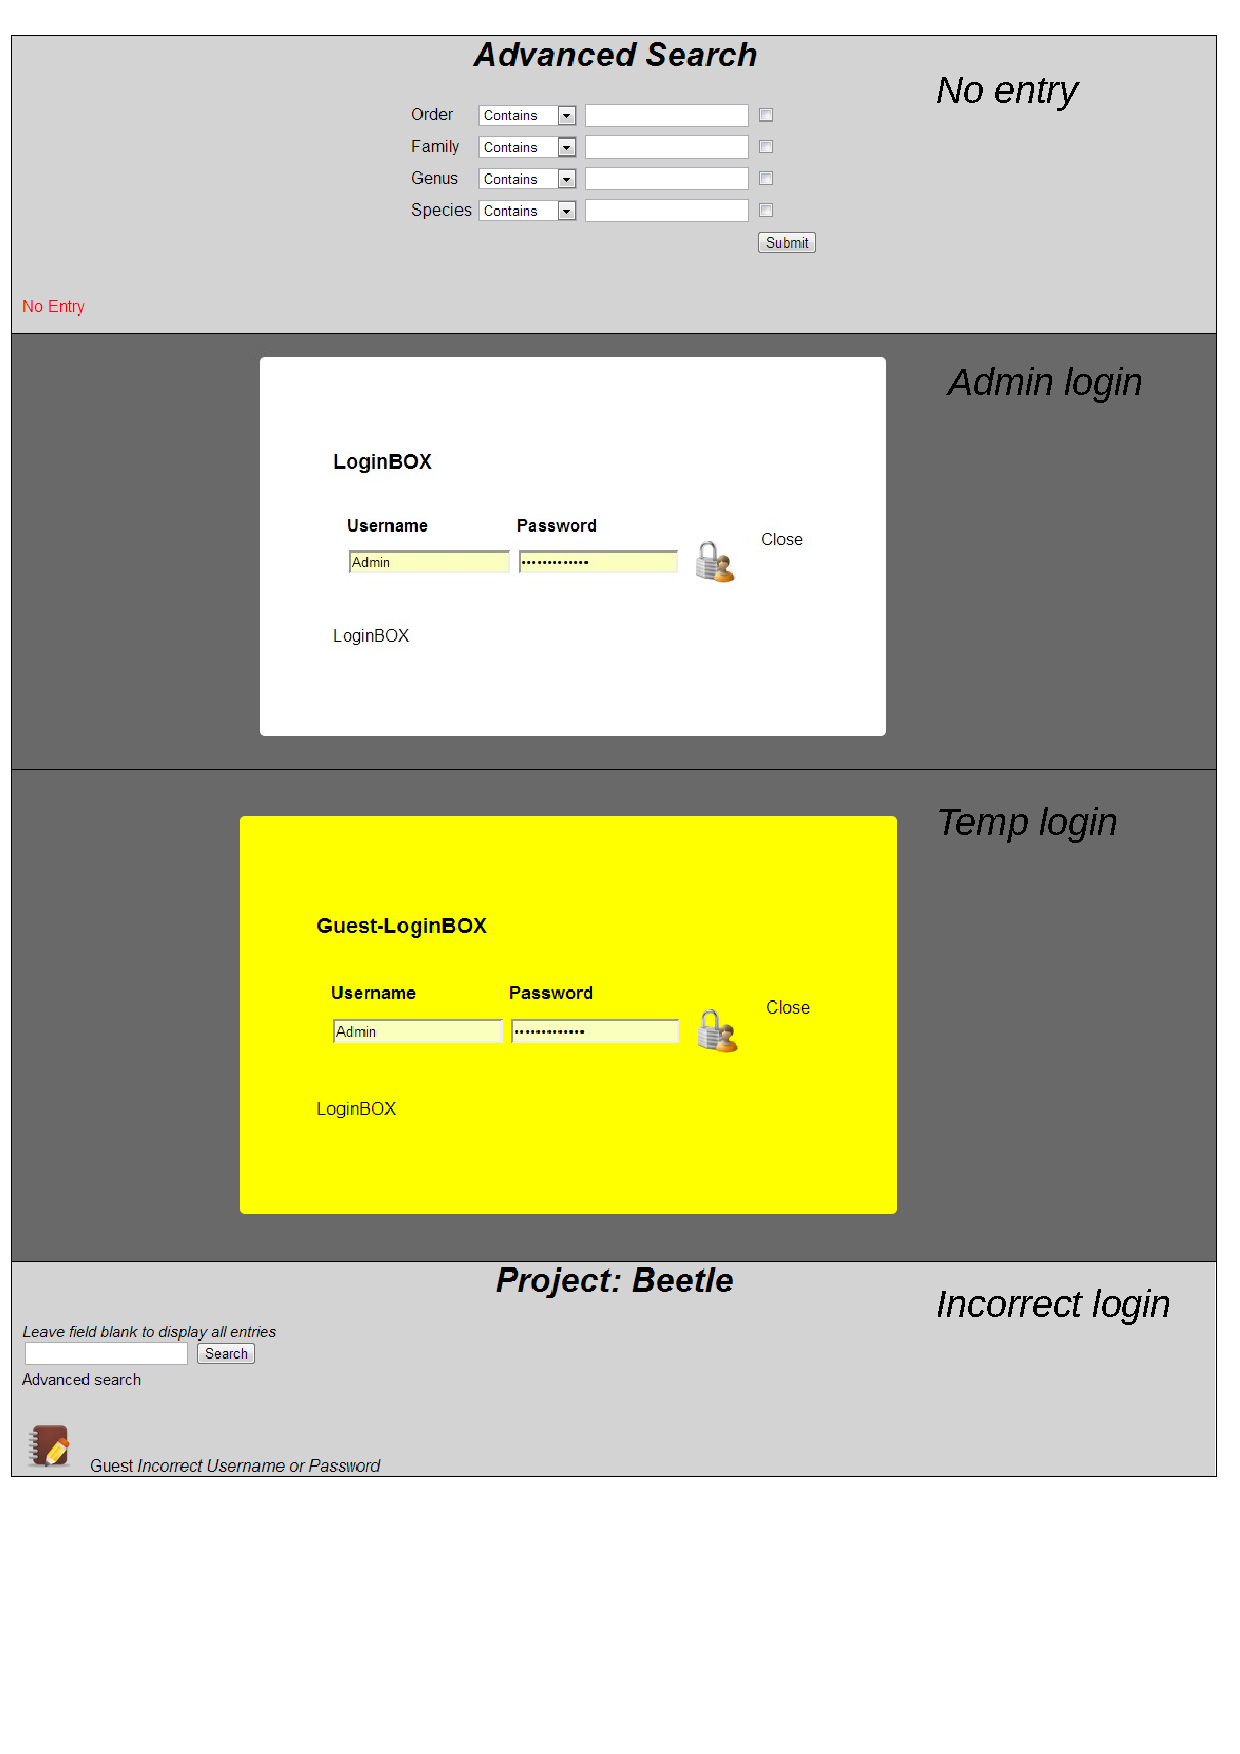
\includegraphics[height=225mm]{UI2.pdf}
\newpage
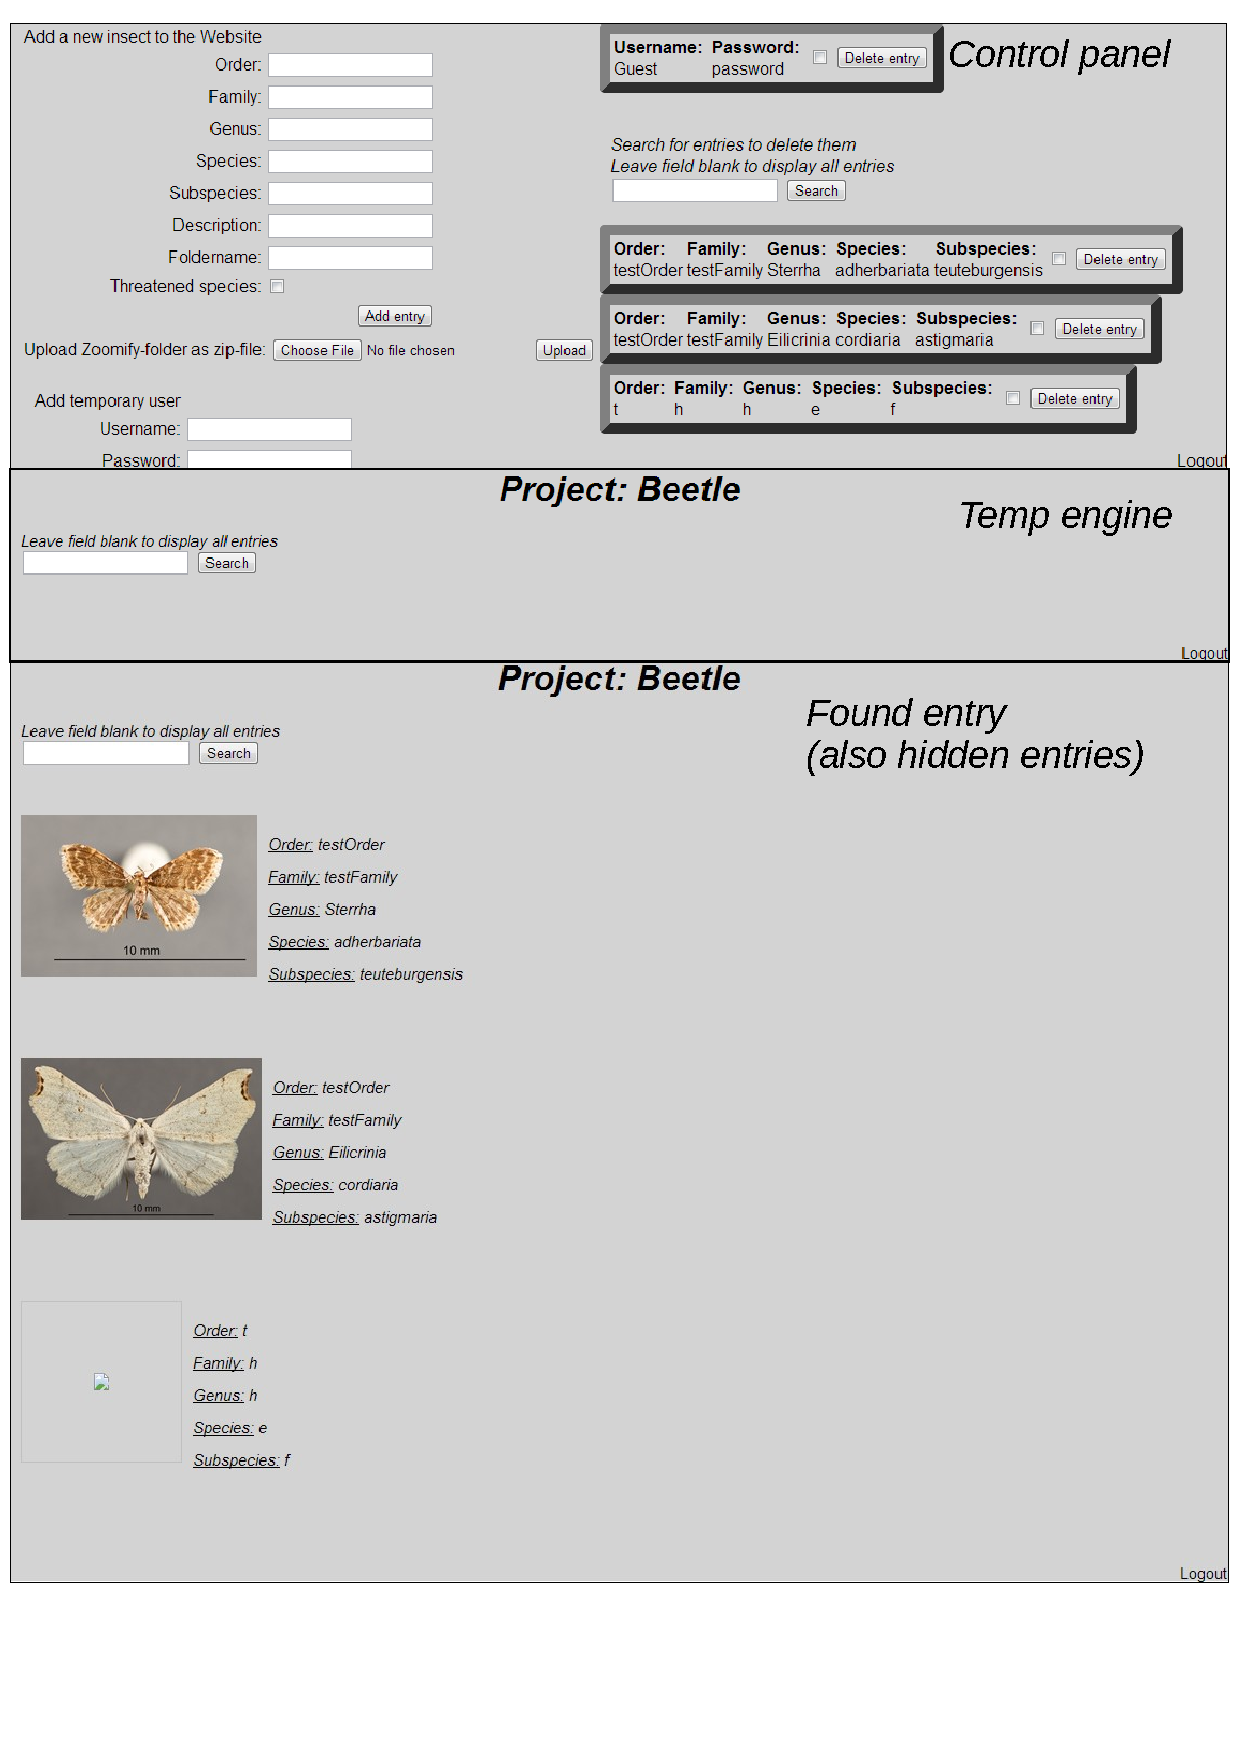
\includegraphics[height=225mm]{UI3.pdf}\\
In addition to these screenshots, a video has also been recorded which showcases the functionality of the website. It can be found at: \url{https://www.youtube.com/watch?v=pAkcdgJnbgc}



\newpage

\section{Internal Cooperation}
\subsection{Summary}

{\bf 22nd of April:}

Come thus far, the cooperation of the University of Hamburg is satisfactory.\\
We have had a total of 2 "official" correspondences with our client in order to formally request server-access and the information we will be needing for the database. Furthermore we have been in contact with the University of Hamburg's Entomology department's representative after every work-session we have had, to present the current state of the product to him.
All the correspondonces have been fulfilling and we will be gaining access to the server as soon as their IT-department have created a user for us.\\ Furthermore, we will be receiving the necessary data for creating the proper database the 22th of April, after which we'll have everything we need. \\
The client also expressed satisfaction regarding the current state of our product, although a desire to have it looking more akin to the current layout of their website (which is only natural given that this is a prototype).\\
Our current way of work is based on us setting up workdays and meetings depending on necessity. This means that we, rather than using a gridlocked schedule, have been deciding on days to meet when the need was expressed.\\
For organisation we have been using a group created in Skype for communication as well as a repository in Github for file-access. \\
We have been internally communicating the progress of the product along the way and have also internally decided which partials have had the most importance at a given point in time, as to ensure we are all on the same page and that deadlines will be met.\\

So far we are making great progress in the development of the product itself, and we will soon have all the available means to ensure a succesful deliverance of a working product.\\
Our effort in organising meetings and working days has been less than ideal and together with our non-gridlock scheduling style have caused us to have many subsequent days of work, causing more of a burden than what is needed.\\
In order to make our developing from here on more efficient, more emphasis will be placed on proper scheduling, in order to spread out the workload and easen the burden on the entire group. This will also allow more time for quality control.\\
\newpage
{\bf 13th of May:}

At this stage the product is fully functional and everything that the University of Hamburg has desired, has been implemented.\\
In regards to our work we continued largely with the approach discussed in the summary from the 22nd of April, in the way that we have been setting up days on which we met and attempted to get as much work done as possible.\\
While we previously discussed the disadvantages to this approach, the progress we had made did not leave a lot of additional work to be completed, and therefore using a predetermined schedule was deemed unnecessary.\\
Our cooperation internally has been more than satisfactory, as each member of the group has been pulling their own assigned work-load, as well as having been constructive with input in regards to the whole project.\\
We have been working more closely with the University of Hamburg, showing them the development of the product underway, and have been continuously involving them in the whole process, so that they could provide their own input on the finished product.\\
The result is, that all their requests have been met satisfactorily, and that we are now almost ready to ship the finished product.

\newpage
\section{Litterature Reviews}
\subsection{Programming as theory building - Peter Naur}
In 1985 Peter Naur gave a brilliant example on how programming and software research should be approached. The general idea is that programmming is theory. This theory is the backbone of all future programs. The point is not to code something specific, the code is not the important thing. Code changes because of demands, optimization etc. It might be the best way to code for 10 years, but after that who knows? Peter Naur said in his abstract that \textit{"(...) it is concluded that the proper, primary aim of programming is, not to produce programs, but to have the programmers build theories of the manner in which the problems at hand are solved by program execution."} \\
The real goal of the software development crew, is not to code something, but to understand the concept behind it. Understanding it rather than just coding something that works makes it easier to solve and develop new solutions. If a theory around your software is created it will make optimization, expansion or modifications easier. Peter Naur even claims that code standing by itself is dead, even though it may be useful for some situations. One quote specifically explains the point of programming:\\ \textit{"Revival of a program is the rebuilding of its theory by a new programmer team"}.\\
Naur also says that documentation is not an appropriate mechanism to transmit knowledge in software projects. In general the idea is that Peter Naur believes that software development isn't about developing software, but more about developing a shared understanding of the software development.
\\
What we can take with us in our project is that we need to understand what we are doing. We need to think about all the modifications, optimizations and requests that the owner might call for. That is why we simply cannot write some code that works, but we don't understand the principle behind it. We need to have a backbone, something we can lean on when we the need for modifications hits us. Since our project was fairly simple we automatically counted in the need for future development, making it easy to expand. But this is not mostly due to our work, but because the project doesn't have many strings to play on. It's a search engine, that works with a specific algorithm that retrieves elements from a database. The idea here is pretty simple, and so is the theory behind it. One thing we can consider is not analyzing what a program is doing, we should analyze how does it take part and affect in the environment it is executed. How the users feel, how different systems work with it. Programming is about working in teams, and in order for a team to work together, all must understand the same theory behind the project.
\newpage
\subsection{XP - Highsmith}
The article is about a style of programming some parts of the community uses. It is called extreme programming and it is a discipline of development bases on simplicity, communication, feedback, courage and respect. The whole team/crew is brought together to do simple tasks, where the feedback is thorough enought to enable the team to see where they are at a current state but also to pinpoint the practices to be able to solve their task. XP is about planning and tracking what to should be done next and to predict the deadline of the project, hence when the project will be finished. The idea is that the extremoes focus on the business that hires them, making sure that they release small portions every now and then, which pass all the tests and demands the customer has defined. This is achieved in pair programming, or in larger groups, with a fairly simple design, and code next to perfect. The group or pair then continuosly work on improving this design and code, just enough to match their current needs or the customers needs. The system never stops running, it is integrated all the time. All the code for production is written in pairs, meaning that the pair / group always work together. They code in a style everyone can understand and improve as they move forward. This makes so that the team has the responsibility for all the code, since the pattern makes so that everyone can understand everyone's code. The group has a common view on how the system looks like, and everyone makes sure they work in a pace which they can sustain for longer periods of work. \\
XP Programmers make sure that they continuosly test their project with their customers. They always want to have a visual software, which is given to the customer in the end of every iteration of work. Besides the XP programmers release frequently. \\
One thing we will close this article off with is the use of pair programming. The idea that two people sit side by side all the time, coding and working on the same computer all day every day. The idea comes from studies showing that pairing produces better code in about the same as programmers working alone. It is literally the idea that two heads really are better than one.\\
\\
In our assignment we have somewhat the same. The urge and need for testing with the client is not that important for our client, but we always want the client to see what we have accomplished. Doing so we have had a front end, a visual representation, from day one, making sure that customer always has something to look at and something to pinpoint. Chances are that they know jack about code, so a visual representation really helps clients. The pair programming aspect is something we have somewhat incorporated since we agreed on the fact that 4 people sitting with their own computer and coding the same things wouldn't benefit in any way other than mixing the different files up. It has generally been two people doing one thing, whilst the other two do another thing. We work with a simple design, and before we started we made it clear what our goal was, and had a clear idea of what our page would look like in the end. This simple design we all had imagined can be seen our webpage to this date, where small adjustments has lessened the work load but also helped us making the site easier to use. It is a search engine - nothing more, nothing less. 

\newpage

\newpage
\section{Annexes}

\subsection{Testing}
Test plan: \\
We want to test the general functionality of our product. The searchfunction is the most important part of the product, followed by the option to add an entry to the database. When those two functions work we can add more functions to the product, like the advanced search and the deletion of an entry in the database.\\\\
Test specification:\\
It should not be hard to test these functions, because we easily can test if the search gives the right output. The add and delete functionality should also be easy to test, because of its easy of use.\\
Testing the search could happen with the mentioned words and letters form section 5. Also we need to test the add entry and delete entry. Here we create a new entry, fitting to a Zoomify-image, and see if it works as intended. After that we could delete that entry again.\\\\
Test incident report:\\
Right now is there one bug in the code: If you login and logout, and go back in the browser you will go back to the edit page. Some could argue, that it is not that bad, because of the user has been logged in before already, but its still a bug that has to be fixed.\\\\
Test summary report:\\
We have tested our product a lot. But there is not much to test; a searchfield, an advanced-search, an add entry function and a delete entry function. Maybe you could count the add Zoomify-image in too, but we count it under the add function.\\
Until now did all tests work out fine. We could use the searches and get a working result. We could add and delete entries. And we could also add a new Zoomify-image-folder to the server.
\newpage
\subsection{Github Log}
\noindent\makebox[\linewidth]{\rule{16.5cm}{0.4pt}}
commit 8b20be842e7ca59aae72ecfce593dd778557bbef
Author: Arcaedes <casper.lutzhoft@gmail.com>
Date:   Tue Jun 2 00:24:04 2015 +0200

Report update

Missing commit log, flow-diagram, some testing stuff and the YouTube
video

commit 4577a9e9206e201af0fc710b2b7de0a6965abe6c
Author: gol1c <enesgolic@live.dk>
Date:   Mon Jun 1 22:44:24 2015 +0200

Reviews final!

commit 1998637a88ad45fb73d849a36549fa09b672e275
Author: gol1c <enesgolic@live.dk>
Date:   Mon Jun 1 20:20:01 2015 +0200

Current Progress of the report v2

Added Sequence diagrams. Added BCE and description. Added Class Diagram
with description.
Added Review of Peter Naur's text

commit fdc578f2ad24b14117933608cfd003ccbb3bf975
Author: TorSalve <torsalve.dalsgaard@yahoo.de>
Date:   Mon Jun 1 16:16:22 2015 +0200

commit log

note to self: git shell ->
git log > log.txt

commit 40204ffe9ce061bfac294dd88706b8ff56a6ba67
Author: TorSalve <torsalve.dalsgaard@yahoo.de>
Date:   Mon Jun 1 15:58:13 2015 +0200

Changelog delraport4

commit 675c39836aa2571093c5c1f3207114a2a48e7cb4
Author: Arcaedes <casper.lutzhoft@gmail.com>
Date:   Mon Jun 1 12:55:42 2015 +0200

Current progress of report.

Updated Abstract, FACTOR, functional requirements, Use-case diagram,
specific use-cases, class-diagram and a lot of text.

commit 195c0a39d9634e79a6fca7dfaa56f11c409c8105
Author: Arcaedes <casper.lutzhoft@gmail.com>
Date:   Wed May 13 01:39:27 2015 +0200

Newest version of report

The newest version of the current report - only missing litterature
reviews and commit-log

commit f9339cf68b8dda5f980168a77b2d7f9ce604c808
Merge: 2006134 a53631f
Author: Arcaedes <casper.lutzhoft@gmail.com>
Date:   Wed May 13 00:58:47 2015 +0200

Merge branch 'master' of https://github.com/yunus73/PROJECT-BEETLE

commit a53631f150dd4b5a2409e2e9d479b71cb99c95b0
Author: TorSalve <torsalve.dalsgaard@yahoo.de>
Date:   Tue May 12 11:49:17 2015 +0200

Underskrift på PAD

commit 6434af45e72392dab6c3f401fef5465cf545cb50
Author: TorSalve <torsalve.dalsgaard@yahoo.de>
Date:   Tue May 12 11:44:52 2015 +0200

Test og -bilag

commit 4cd0fdc87fe731176b8d145f8550e109e1fa1497
Author: TorSalve <torsalve.dalsgaard@yahoo.de>
Date:   Mon May 11 21:04:10 2015 +0200

Changelog

commit bd3b4eba5f5aa239041215ab111d2d0bae4d4489
Author: TorSalve <torsalve.dalsgaard@yahoo.de>
Date:   Mon May 11 18:21:28 2015 +0200

Project Agreement Definition

PAD for the costumer

commit 20061346a0c24845a210b70a8354393f54bf563f
Author: Arcaedes <casper.lutzhoft@gmail.com>
Date:   Wed Apr 22 01:34:06 2015 +0200

Finished version of report 2!

All models and descriptions added, will upload the report shortly.

commit e93c13891bb4264b7d0a729a14d5be02105f79aa
Author: yunus73 <yun933141@gmail.com>
Date:   Wed Apr 22 01:24:42 2015 +0200

Updated BCEMODEL

commit 75f7cadce41820ca3cc82e31ffad9b3fbaabd98d
Author: Arcaedes <casper.lutzhoft@gmail.com>
Date:   Wed Apr 22 00:59:54 2015 +0200

Almost finished version of the report.

Only the BCE-diagram is missing.

commit d6be929036b7d326017adc96a4d680b09ff6c180
Author: yunus73 <yun933141@gmail.com>
Date:   Wed Apr 22 00:59:00 2015 +0200

BCEMODEL

commit bb6a58e6dcc960b80874ef0f20a69f3c22d2d997
Author: gol1c <enesgolic@live.dk>
Date:   Wed Apr 22 00:39:22 2015 +0200

Diagrams

3 Use Cases and 1 Class Diagram

commit 87c8d0e13cc2c07cf6d31e6ddd19bb1b031f89dc
Author: TorSalve <torsalve.dalsgaard@yahoo.de>
Date:   Wed Apr 22 00:16:18 2015 +0200

log

commit a2f101fd1d53f2a48a609b4248973931d2246762
Author: Arcaedes <casper.lutzhoft@gmail.com>
Date:   Tue Apr 21 23:59:23 2015 +0200

Newest version of report 2.

Added the litterature reviews and changed some stuff around/added some
stuff here and there.

commit 0e78c2f140753bee0c9d81675f9a4be3b8b80b62
Author: TorSalve <torsalve.dalsgaard@yahoo.de>
Date:   Tue Apr 21 23:57:55 2015 +0200

timeline/new changelog

commit 36289677a765ca0b1233cd127c299446420a61f6
Author: gol1c <enesgolic@live.dk>
Date:   Tue Apr 21 23:25:24 2015 +0200

Reviews

Reviews of the two papers.

commit af1ee59f4b9ab9719db1f286b4ac88934b22cf85
Author: gol1c <enesgolic@live.dk>
Date:   Tue Apr 21 23:24:08 2015 +0200

okok

Skal åbenbart commite før jeg can synce. DONT USE THIS

commit 696e4999ede32af3353b7b76f32b9f7d50d14e85
Author: TorSalve <torsalve.dalsgaard@yahoo.de>
Date:   Tue Apr 21 23:10:41 2015 +0200

Added new changelog and code

commit 7757964b1829bbb72615b62835f3865b36c4eb94
Author: Arcaedes <casper.lutzhoft@gmail.com>
Date:   Tue Apr 21 23:02:28 2015 +0200

Current state of the report.

This is the current state of partial report 2, still missing some
points.

commit f7b07df6661d4d4e7b28feded204a7b24f27b559
Author: TorSalve <torsalve.dalsgaard@yahoo.de>
Date:   Tue Apr 21 22:36:35 2015 +0200

ChangeLog 20-21.04

commit 298c0df1a827d7abe8e8f64ab4dbfcae728814fd
Author: TorSalve <torsalve.dalsgaard@yahoo.de>
Date:   Tue Apr 21 21:19:00 2015 +0200

cleanUP

commit 5370d72b85a93d892e3ab1788d7b54f288c55842
Author: yunus73 <yun933141@gmail.com>
Date:   Tue Mar 31 22:35:43 2015 +0200

Mjallo virkelig ny

commit b0eee357d0624164d6b055d0f920a88be07eeee4
Author: yunus73 <yun933141@gmail.com>
Date:   Tue Mar 31 21:00:36 2015 +0200

Mjallo ny

commit 3045fee9ccf70078c5da93925c67dff383287c11
Author: yunus73 <yun933141@gmail.com>
Date:   Tue Mar 31 21:00:12 2015 +0200

Mjallo

commit 5726df9712cd379e4bf1852277a81859f64b38eb
Merge: db797ee 8ee517f
Author: Arcaedes <casper.lutzhoft@gmail.com>
Date:   Tue Mar 31 20:46:45 2015 +0200

Merge remote-tracking branch 'origin/master'

Conflicts:
Delrapport 1/1 opgaver.log
Delrapport 1/1 opgaver.pdf
Delrapport 1/1 opgaver.synctex.gz

commit db797ee5d68ac6723f919d152a86b9033875327a
Author: Arcaedes <casper.lutzhoft@gmail.com>
Date:   Tue Mar 31 20:45:16 2015 +0200

Fixed it!

commit 8ee517f6998900948287d6f762d72902b5f959ce
Author: yunus73 <yun933141@gmail.com>
Date:   Tue Mar 31 20:45:10 2015 +0200

try tis

commit ebe615ae222932117f361dcfa6db94c4e96caaaa
Author: Arcaedes <casper.lutzhoft@gmail.com>
Date:   Tue Mar 31 19:35:32 2015 +0200

Edited the report.

Logo added, Problem Statement changed.

commit 339fa41b0ea5833d997d0a3156fa393f777a91c2
Author: Arcaedes <casper.lutzhoft@gmail.com>
Date:   Tue Mar 31 18:41:37 2015 +0200

Report + Pictures

Missing file KULogo.pdf to compile.

commit 0d21845509f086db663ddd3e1f9bc837a48431f0
Author: gol1c <enesgolic@live.dk>
Date:   Mon Mar 30 11:42:09 2015 +0200

Delrapport 1- rettelse 1

Der mangler stadig meget at skulle rettes drenge. Jeg kan ikke lave mere
nu, har ikke mere materiale til rådighed nu.

Skriv til mig, vi skal have lavet det her.

commit c129a2c8d39a08817ae8b1af6f4e66e52b70c8e3
Author: yunus73 <yun933141@gmail.com>
Date:   Mon Mar 30 22:03:00 2015 +0200

Killefilder

Mjallo

commit b0d9a30e25ab130b74aae20dfc13751086fad25d
Author: yunus73 <yun933141@gmail.com>
Date:   Mon Mar 30 21:56:40 2015 +0200

Scheduleplan

Mjallo

commit c477a2f0b1cd43f3e8c5f5fad3ee5610d45ec5a9
Author: yunus73 <yun933141@gmail.com>
Date:   Mon Mar 30 21:02:24 2015 +0200

Skillmatrix

mjallo

commit 57514365ae01e66fc840a1a83a9179da99af024b
Author: TorSalve <torsalve.dalsgaard@yahoo.de>
Date:   Wed Mar 25 18:14:21 2015 +0100

review of the review

commit 6d0c506dba8431f54e9981bc898c830886223327
Author: gol1c <enesgolic@live.dk>
Date:   Wed Mar 25 17:48:33 2015 +0100

Echo delrapport

commit 0df006f92077a6b459be84ea12024602cf1d2085
Author: gol1c <enesgolic@live.dk>
Date:   Wed Mar 25 02:37:06 2015 +0100

Feedback til Project Echo

commit f2cdb6502564f898d552c8f5155ea625e0bad597
Author: TorSalve <torsalve.dalsgaard@yahoo.de>
Date:   Tue Mar 24 18:28:19 2015 +0100

.tex-filer 4 you

commit 783af0a7dd52a49736377bcf7fcad341bd6ae45b
Author: TorSalve <torsalve.dalsgaard@yahoo.de>
Date:   Mon Mar 23 13:28:59 2015 +0100

Redone the enviroment

Sort after lort

commit 16bfea5826fec94696e582579f37c8fd2ec56984
Author: Arcaedes <casper.lutzhoft@gmail.com>
Date:   Mon Mar 23 13:08:08 2015 +0100

English corrections/changes

English part of the document

commit 5c8451d83064b0c0b29857c8f75712a86f11ebb4
Author: TorSalve <torsalve.dalsgaard@yahoo.de>
Date:   Mon Mar 23 11:54:57 2015 +0100

Changed the name

Because Yunus cant do it proper

commit dd63eb090704d7f502b7b79397047ad4976ad58e
Author: yunus73 <yun933141@gmail.com>
Date:   Mon Mar 23 11:50:20 2015 +0100

Hermaen

commit 6b0723be7163a375c2a9a2e5359a777d04aaa285
Author: TorSalve <torsalve.dalsgaard@yahoo.de>
Date:   Sat Mar 21 12:26:27 2015 +0100

delrapport 1 assignments

commit be9faa6af526e161f19e2c7ad3d64877d004d380
Author: TorSalve <torsalve.dalsgaard@yahoo.de>
Date:   Sat Mar 21 12:10:43 2015 +0100

1.6/1.8

commit 078727206a345068ad71637c608e7fd16257f130
Author: TorSalve <torsalve.dalsgaard@yahoo.de>
Date:   Sat Mar 21 11:47:48 2015 +0100

Clean up!

commit 00a67141008584aed46537f9fe63f2aa2e6e86a7
Author: TorSalve <torsalve.dalsgaard@yahoo.de>
Date:   Fri Mar 20 17:18:18 2015 +0100

delete double

commit 4f6a322e51e9abd238f07aa975d4f35f594cd50a
Author: gol1c <enesgolic@live.dk>
Date:   Fri Mar 20 16:53:51 2015 +0100

Projekt Etablering

commit d20a46817e08e7613bc7a6b16d668e48cebc7b63
Author: Arcaedes <casper.lutzhoft@gmail.com>
Date:   Fri Mar 20 16:52:29 2015 +0100

Rewrote the description

commit 96050dbd1e2b98be793fcd90607a0d36cefaba0a
Author: Arcaedes <casper.lutzhoft@gmail.com>
Date:   Fri Mar 20 16:39:51 2015 +0100

Statements and Project Agreement Definition

The finished initial statements of our rapport as well as the initial
issue of the Project Agreement Definition.

commit da46259144ba11472c71b59d9b5a23039996858c
Author: yunus73 <yun933141@gmail.com>
Date:   Fri Mar 20 16:35:21 2015 +0100

Hello

commit 4c5850dbebe4dc945c52d14bdcdd7d123677ace1
Author: TorSalve <torsalve.dalsgaard@yahoo.de>
Date:   Fri Mar 20 16:16:09 2015 +0100

Initial Software Architecture (updated)

commit fa8824f3801c8de0b346d385762fc8a090485a2e
Author: TorSalve <torsalve.dalsgaard@yahoo.de>
Date:   Fri Mar 20 15:02:58 2015 +0100

Initial Software architecture

commit 906e4ca7670e3a2340423a03b92635f3627a5041
Author: TorSalve <torsalve.dalsgaard@yahoo.de>
Date:   Fri Mar 20 14:57:34 2015 +0100

Initial SPMP

commit 0789c6f12293fd05c1f67e31535fbac089ec5b3d
Author: Arcaedes <casper.lutzhoft@gmail.com>
Date:   Fri Mar 20 14:38:12 2015 +0100

Introductory/Problem statement

The first 2 statements to our report.

commit acb432477ecd86315b4c18059172ae99569b6194
Author: TorSalve <torsalve.dalsgaard@yahoo.de>
Date:   Fri Mar 20 14:35:26 2015 +0100

7.1 Deployment Diagram

commit bfcbd73bef6e603b15e7f22c90d21abc6e22304f
Author: gol1c <enesgolic@live.dk>
Date:   Fri Mar 20 14:29:55 2015 +0100

sup

commit 9efec634675f963b5455292637582147676a557b
Author: gol1c <enesgolic@live.dk>
Date:   Fri Mar 20 14:01:05 2015 +0100

Revert "HEJ YUNUS"

This reverts commit 707601f0da6d54a88530306be6251417eb5e39b4.

commit 13eef8153adf3e5c672ee19713b009108c0d0200
Author: gol1c <enesgolic@live.dk>
Date:   Fri Mar 20 13:59:46 2015 +0100

HEJ YUNUS

YUNUS IS HAIRY

commit 0851690c2269aa1347c9af60231434a85ed71df1
Author: yunus73 <yun933141@gmail.com>
Date:   Fri Mar 20 13:54:19 2015 +0100

Hello Casper

Casper is VERY BALD

\noindent\makebox[\linewidth]{\rule{16.5cm}{0.4pt}}

The code at this point in time have been developed in cooperation with the entire group through meetings at the school, where we worked on the code on only a single computer. As such, the Github log will not bear trace of editing of the code. The line 696e499 however shows the addition of the beta-version's code to the project's folder.
\newpage
\subsection{Changelog}

	$$
	\begin{array}{lrl}
	\bf{Date}~&~\bf{Name}~&~\bf{Change}~\\~
	20-04-15~&~YO/TD/EG/CL~&~Added~seachfield~and~\text{-}button~\\
	20-04-15~&~YO/TD/EG/CL~&~Added~database~and~entries~\\
	20-04-15~&~YO/TD/EG/CL~&~\vtop{\hbox{\strut~\emph{Added~edit\-link}}}~\\
	21-04-15~&~YO/TD~&~\vtop{\hbox{\strut~\emph{Added~Family\text{-},~Genus\text{-}~and~Species\text{-}names~form~the~database}}\hbox{\strut~\emph{to~the~webpage}}}~~\\~
	21-04-15~&~YO/TD~&~Added~picture~of~the~found~insect(s)~\\
	21-04-15~&~TD~&~Added~CSS\text{-}code~to~shine~the~webpage~a~bit~up~\\
	21-04-15~&~TD~&~Updated~the~database,~so~it~actually~shows~an~actual~insect\\
	21-04-15~&~TD~&~Added~Order\text{-}name\\
	01-05-15~&~TD~&~Added~Zoomify~pictures~and~the~description~of~the~insect\\
	01-05-15~&~YO~&~Added~login\\
	11-05-15~&~TD/CL~&~\vtop{\hbox{\strut~\emph{	Added~option,~for~an~employee,~to~add~a~new~entry~into~}}\hbox{\strut~\emph{the~database}}}~\\
	11-05-15~&~TD/CL~&~\vtop{\hbox{\strut~\emph{	Added~option,~for~an~employee,~to~delete~an~old~entry~from}}\hbox{\strut~\emph{the~database}}}~\\
	11-05-15~&~CL~&~\vtop{\hbox{\strut~\emph{	Added~feature,~that~displays~all~entries,~when~the~search\text{-}}}\hbox{\strut~\emph{~field~is~blank}}}\\
	11-05-15~&~YO/EG~&~Added~functionality~for~the~advanced~search\\
	01-06-15~&~YO~&~Fixed~issue~with~cookies/cache~\\~
	01-06-15~&~YO/EG~&~Added~temporary-login~\\~
	01-06-15~&~YO~&~Fixed~the~temporary-login~so~i~works~as~intended~\\~
	01-06-15~&~TD/EG~&~Edited~editpage,~so~the~admin~can~add~new~temporary~users~\\~
	01-06-15~&~TD~&~Edited~editpage,~so~the~admin~can~mark~an~entry~as~hidden~\\~
	01-06-15~&~TD~&\vtop{\hbox{\strut~\emph{	~Edited~editpage,~so~the~admin~can~look~up~entries,~to~make~it~}}\hbox{\strut~\emph{easier~to~delete~entries}}}\\~
	02-06-15~&~CL~&~Revamped~the~entire~report~and~added~video
	\end{array}
	$$
\subsection{Timeline}

	Initial custommer contact - {\bf 12th of March} - The custommer explained the desired functionality for the search-engine and their expectations of the outcome of the project. \\
	
	
	Report 1 - {\bf 21st of March} - The custommer received a copy of our first report, in order for them to view our progress and method of work.
	The custommer here expressed their desire for a more advanced option of using the search-engine. The exact specifics of what this should contain have not yet been stated, but they said they'd get back to us.
	They also expressed their desire for a dropdown menu showcasing all the entries in the database, in order to give the visitors a better overview.\\
	
	
	Prototype - {\bf 21st of April} - The custommer was officially shown the prototype of our search-engine, and they approved of its design. They pointed out some modifications that had to be made, most notably the correcting the attributes and wanting a new attribute, order, added. The correct order of attribute entries have now been specified as order, family, genus and species.\\
	
	Finished product - {\bf 11th of May} - On this date all functionality missing from the website was implemented and tested, so that we would end up with a product that (apart from a particular bug) is complete.\\
	It was also shown to the University of Hamburg, where they expressed great satisfaction with our product, and also the way we provided the option for displaying all entries, even prefering it to the one they had originally desired.\\
	
	Additional functionality - {\bf 2nd of June} - Leading up to this date, a lot of additional functionality has been added to the product.\\
	For starters, it is now possible to mark entries as "threatened", which will hide them in the public search-engine and only make them available to people with a temporary login.\\
	\\Furthermore the administrator function to add a temporary user has also been added to the product, which is now fully operational and meets all the criterias set by the University of Hamburg.



\end{document}
